\documentclass[english,dvipdfmx]{jsarticle}
\usepackage{amsmath,amssymb}
\usepackage{color}
\usepackage[hiresbb]{graphicx}
\usepackage{multirow}
\usepackage{tabularx}
\usepackage{here}
\newcommand{\average}[1]{\ensuremath{\langle#1\rangle} }
\newcommand*{\point}{\textcircled{\textcolor{red}{\scriptsize キ}}}
\newcommand*{\proof}{\textcircled{\textcolor{blue}{\scriptsize P}}}
\begin{document}
\section{Topological space}
\begin{description}
    \item[\bf{Definition:}] Characterizations of the category of topological space
        \begin{enumerate}
            \renewcommand{\labelenumi}{(\Roman{enumi}).}
            \item Definition via open sets (開集合系) \\
                all pairs $( X,\ \mathfrak{O})$ of set $X$ together with a collection $\mathfrak{O}$ of subsets of $X$ satisfying:
                \begin{enumerate}
                    \renewcommand{\labelenumii}{\arabic{enumii}.}
                    \item $\phi,\ X \in \mathfrak{O}$
                    \item $ (O_{\lambda})_{\lambda \in \Lambda},\ |\Lambda| < \aleph_0,\ \forall \lambda \in \Lambda ( O_{\lambda} \in \mathfrak{O} ) \Rightarrow \cup_{\lambda \in \Lambda} O_{\lambda}  \in \mathfrak{O}$
                    \item $ (O_{\lambda})_{\lambda \in \Lambda},\ \forall \lambda \in \Lambda ( O_{\lambda} \in \mathfrak{O} ) \Rightarrow \cap_{\lambda \in \Lambda} O_{\lambda}  \in \mathfrak{O}$
                \end{enumerate}

            \item Definition via closed sets (閉集合系) \\
                all pairs $( X,\ \mathfrak{C})$ of set $X$ together with a collection $\mathfrak{C}$ of subsets of $X$ satisfying:
                \begin{enumerate}
                    \renewcommand{\labelenumii}{\arabic{enumii}.}
                    \item $\phi,\ X \in \mathfrak{C}$
                    \item $ (C_{\lambda})_{\lambda \in \Lambda},\ \forall \lambda \in \Lambda ( C_{\lambda} \in \mathfrak{C} ) \Rightarrow \cup_{\lambda \in \Lambda} C_{\lambda}  \in \mathfrak{C}$
                    \item $ (C_{\lambda})_{\lambda \in \Lambda},\ |\Lambda| < \aleph_0,\ \forall \lambda \in \Lambda ( C_{\lambda} \in \mathfrak{C} ) \Rightarrow \cap_{\lambda \in \Lambda} C_{\lambda}  \in \mathfrak{C}$
                \end{enumerate}

            \item Definition via interior operators (開核作用子) \\
                all pairs $( X,\ int)$ of set $X$ together with ans interior operator $int : \mathfrak{P}(X) \rightarrow \mathfrak{P}(X)$ satisfying:
                \begin{enumerate}
                    \renewcommand{\labelenumii}{\arabic{enumii}.}
                    \item $int(\phi) = \phi \quad ( \Leftrightarrow int(X) = X )$
                    \item $\forall M \in \mathfrak{P}(X),\ int(M) \subset M$
                    \item $\forall M,N \in \mathfrak{P}(X),\ int(M \cap N) = int(M) \cap int(N)$
                    \item $\forall M \in \mathfrak{P}(X),\ int(int(M)) = int(M)$
                \end{enumerate}
            \item Definition via closure operators (閉包作用子) \\
                all pairs $( X,\ cl)$ of set $X$ together with ans closure operator $cl : \mathfrak{P}(X) \rightarrow \mathfrak{P}(X)$ satisfying:
                \begin{enumerate}
                    \renewcommand{\labelenumii}{\arabic{enumii}.}
                    \item $cl(\phi) = \phi \quad ( \Leftrightarrow cl(X) = X )$
                    \item $\forall M \in \mathfrak{P}(X),\ M \subset cl(M)$
                    \item $\forall M,N \in \mathfrak{P}(X),\ cl(M \cup N) = cl(M) \cup cl(N)$
                    \item $\forall M \in \mathfrak{P}(X),\ cl(cl(M)) = cl(M)$
                \end{enumerate}
            \item Definition via neighbourhoods (近傍系)
                all pairs $( X,\ V)$ of set $X$ together with a neighbourhood function $V : X \rightarrow \mathfrak{P}(X)$
                \begin{enumerate}
                    \renewcommand{\labelenumii}{\arabic{enumii}.}
                    \item $\forall V \in V(x),\ x \in V$
                    \item $\forall U \subseteq X,\ V \in V(x),\ V \subset U \Rightarrow U \in V(x)$
                    \item $(V_{\lambda})_{\lambda \in \Lambda}, |\Lambda| < \aleph_0,\ \forall \lambda \in \Lambda(V_{\lambda} \in V(x)) \Rightarrow \cap_{\lambda \in \Lambda} V_{\lambda} \in V(x)$
                    \item $\forall V \in V(x),\ \exists W \in V(x): \forall y \in W,\ V \in V(y)$, ( $W = V^i$ meet the requirement. )
                \end{enumerate}
        \end{enumerate}
    
    \item[\bf{Definition:}] Comparison of topologies ( 位相の比較 )
        $$\mathfrak{O}_1 \subset \mathfrak{O}_2 \equiv \text{`` } \mathfrak{O}_1 \text{ is coarser than } \mathfrak{O}_2 \text{ "}\equiv \text{`` } \mathfrak{O}_2 \text{ is finer than } \mathfrak{O}_1 \text{ "},\ ( \mathfrak{O},\ \subset) \text{ is \color{red}{an order set.}}$$
    
    \item[\bf{Definition:}] Topology generation ( 位相の生成 )\\
        Let $X$ be a set, $\mathfrak{X}$ is a subset of $\mathfrak{P}(X)$ i.e. $\mathfrak{X} \subset \mathfrak{P}(X)$
        $$ \text{The corsest topology including }\mathfrak{X}  \text{ is denoted by } \mathfrak{O}(\mathfrak{X}),\text{ it is called the topology generated by }\mathfrak{X}.$$
        The following is how to generate any topology from $\mathfrak{X}$:
        \begin{enumerate}
            \item $\mathfrak{X_0} = \cap U \quad ( U \in \mathfrak{X} )$
            \item $\mathfrak{O}(\mathfrak{X}) = \cup V \quad ( V \in \mathfrak{X_0} )$
        \end{enumerate}
    
    \item[\bf{Theorem:}] the supremum and infimum of topology set
        $$\inf\{ \mathfrak{O}_{\lambda} \mid \lambda \in \Lambda \} = \cap_{\lambda \in \Lambda} \mathfrak{O}_{\lambda} ,\ \sup\{ \mathfrak{O}_{\lambda} \mid \lambda \in \Lambda \} = \mathfrak{O}(\cup_{\lambda \in \Lambda} \mathfrak{O}_{\lambda})$$

    \item[\bf{Definition:}] Induced topology ( 誘導位相 )
        \begin{enumerate}
            \item induced from a set $Y$. \\
            Let $X$ be a set, $( Y,\ \mathfrak{O}_Y )$ be a topological space, $f$ is continuous $X \mapsto Y$. \\
            The induced topology on $X$ is defined by:
            $$\mathfrak{O}_{X} = \{ f^{-1} (U) \mid U \in \mathfrak{O}_{Y}\}$$
            \point \ $f$が連続関数となるように誘導位相$\mathfrak{O}_{X}$定める.$f$が連続となるような$X$の位相の中では最弱.
            \item induced from a collection of sets $( Y_{\lambda})_{\lambda \in \Lambda}$ \\
            Let $X$ be a set, $( Y_{\lambda},\ \mathfrak{O}_{\lambda} )_{\lambda \in \Lambda}$ be a collection of a topology space, $f_{\lambda}$ is continuous $X \mapsto Y_{\lambda}$. \\
            The induced topology on $X$ is defined by:
            $$\sup \{ \mathfrak{O}_{\lambda} \mid \lambda \in \Lambda \} ,\ \mathfrak{O}_{\lambda} = \{ f_{\lambda}^{-1} (U) \mid U \in \mathfrak{O}_{\lambda}\}. $$
            \point \ $f_{\lambda}$が全て連続となるような$X$の位相の中では最弱の位相を求めている.
        \end{enumerate}

    \item[\bf{Definition:}]  Subspace topology ( 部分位相 )\\
        Let $( Y,\ \mathfrak{O}_Y)$ be a topological space, $X$ be a subset of $Y$ i.e. $X \subset Y$ \\
        The subspace topology on $X$ is defined by:
        $$\mathfrak{O}_{X} = \{ U \cap Y \mid U \in \mathfrak{O}_{Y} \}$$
        \point \ 部分集合に与える自然な位相.包含写像による誘導位相.

    \item[\bf{Definition:}] Cartesian topology ( 直積位相 )\\
        Let $( X_{\lambda},\ \mathfrak{O}_{\lambda} )_{\lambda \in \Lambda}$ be a collection of topological space. \\
        The cartesian topology $\mathfrak{O}$ is induced on $\prod_{\lambda \in \Lambda} X_{\lambda}$ by projection $pr_{\lambda} : \prod_{\lambda \in \Lambda} X_{\lambda} \rightarrow X_{\lambda}$.
        The Cartesian topology on $\prod_{\lambda \in \Lambda} X_{\lambda}$ is defined by:
        \begin{eqnarray*}
        & & \sup \{ \mathfrak{O}_{\lambda}^* \mid \lambda \in \Lambda \} = \mathfrak{O}(\cup_{\lambda \in \Lambda} \mathfrak{O}_{\lambda}^*) \\
        & & \mathfrak{O}_{\lambda}^* = \{ pr_{\lambda}^{-1} (O_{\lambda}) \mid O_{\lambda} \in \mathfrak{O}_{\lambda} \} = \prod_{ \iota \in (\Lambda - \lambda)  } X_{\iota} \times O_{\lambda} \quad (O_{\lambda} \in \mathfrak{O}_{\lambda}) 
        \end{eqnarray*}
        \point \ 直積集合に与える自然な位相.射影による誘導位相.
    
    %\item[\bf{Example:}]
    \item[\bf{Definition:}] Quotient space ( 商位相 )\\
        Let $X / R$ be a quotient set, $( X,\ \mathfrak{O}_{X})$ be a topological space, $\pi$ is natural projection $X \mapsto X / R$ \\
        The Quotient space $\mathfrak{O}$ is defined by:
        $$\mathfrak{O}_{X/R} = \{ \pi (U) \mid \pi^{-1}(U) \in \mathfrak{O}_{X}\}.$$
        \point \ 商集合に与える自然な位相.自然な射影による誘導位相.
    
    \item[\bf{Definition:}] Points in topological space.
        \begin{figure}[H]
            \begin{center}
                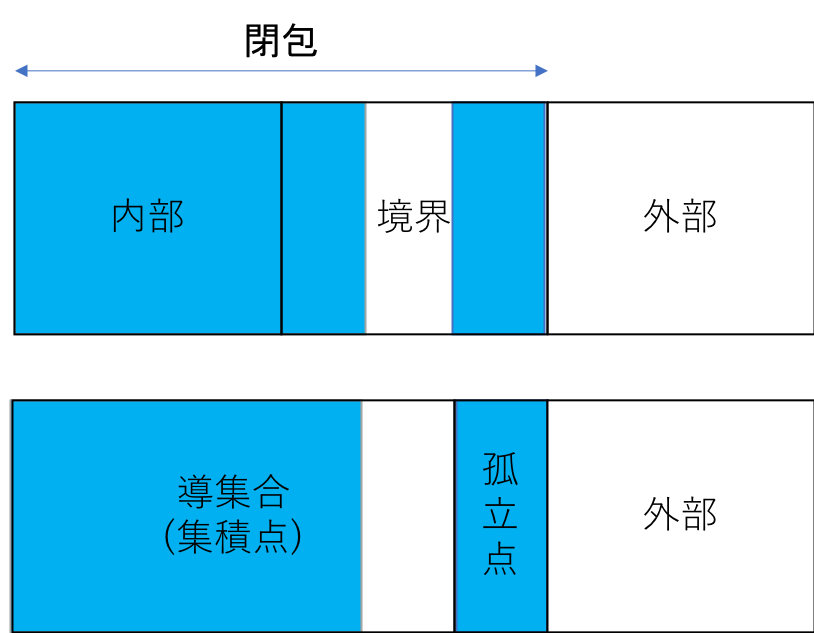
\includegraphics[clip,width=6cm]{./interior.png}
                \caption{Points in topological space}
            \end{center}
        \end{figure}
    
    \item[\bf{Definition:}] Base and Subbase \\
        Let $( X,\ \mathfrak{O})$ be a topological space, $\mathfrak{B}$ be a collection of open set.\\
        The Base is defined by:
            $$\forall O \in \mathfrak{O},\ O = \cup_{\lambda \in \Lambda} B_{\lambda} \quad (B_{\lambda} \in \mathfrak{B}) $$
        Let $X$ be a set, the base of the corsest topology $\mathfrak{O}$ on $X$ including $\mathfrak{B}$ satisfying:
            $$\cup \mathfrak{B} = X,\ \forall B_1,\ B_2 \in \mathfrak{B},\ \exists \mathfrak{B}' \subset \mathfrak{B} \ s.t. \ B_1 \cap B_2 = \cup \mathfrak{B}'$$
        The subbase of the $\mathfrak{O}$ is satisfying:
            $$\cup \mathfrak{B} = X$$

            
        


    \item[\bf{Definition:}] Separation axioms \\
        \point \ 位相が弱すぎないための条件
        \begin{figure}[H]
            \begin{center}
                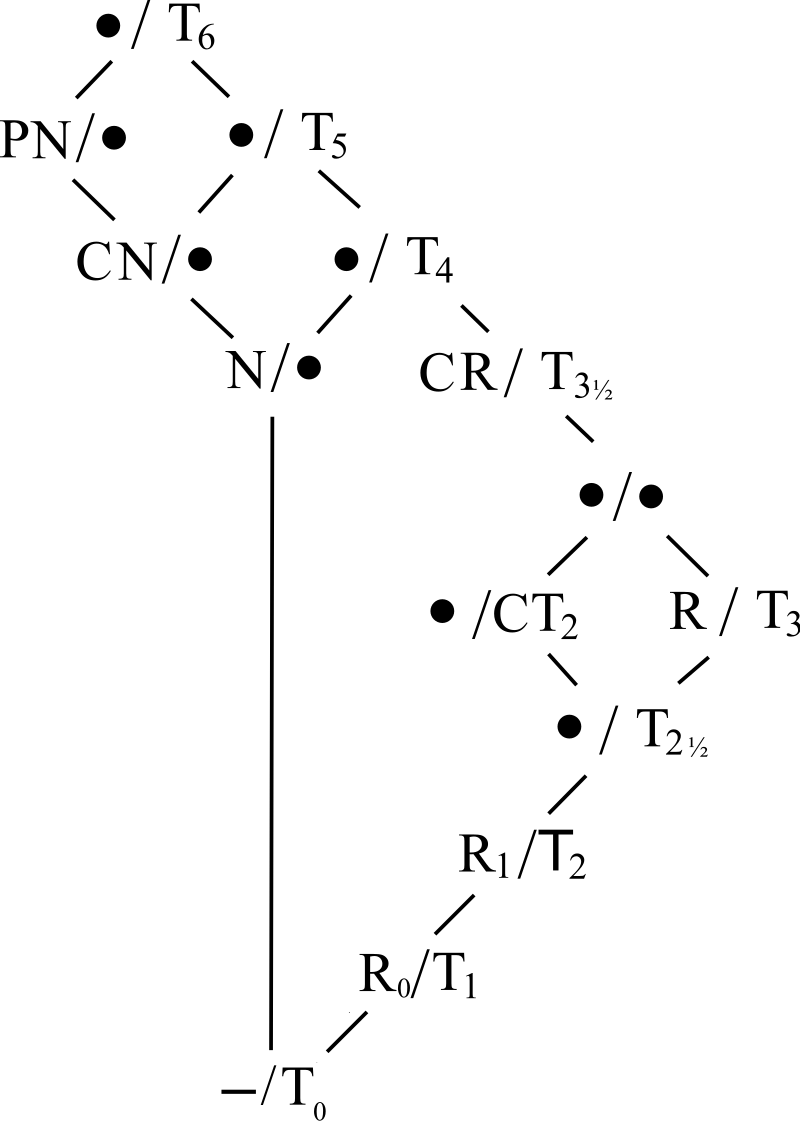
\includegraphics[clip,width=6cm]{./separate_axiom.png}
                \caption{Separation Axioms}
            \end{center}
        \end{figure}
        \begin{enumerate}
            \item $T_0$ : Kolmogorov space $(X,\ \mathfrak{O})$ \\
            $$\forall x,y \in X,\ (\exists V \in V(x) \ s.t. \  x \in V,\ y \notin V ) \lor (\exists V \in V(y) \ s.t. \  x \notin V,\ y \in V )$$
                \begin{figure}[H]
                    \begin{center}
                        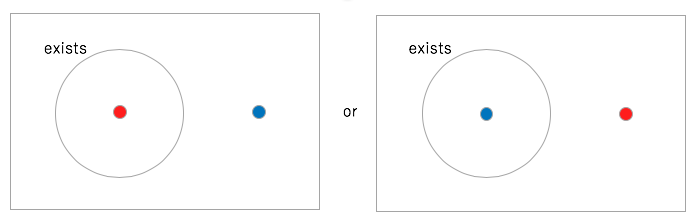
\includegraphics[clip,width=10cm]{./T0.png}
                        \caption{$T_0$ space}
                    \end{center}
                \end{figure}
            
            \item $T_1$ : $T_1$ space $(X,\ \mathfrak{O})$ \\
                $$\forall x,\ y \in X,\ (\exists V \in V(x) \ s.t. \  x \in V,\ y \notin V ) \land (\exists V \in V(y) \ s.t. \  x \notin V,\ y \in V )$$
                \begin{figure}[H]
                    \begin{center}
                        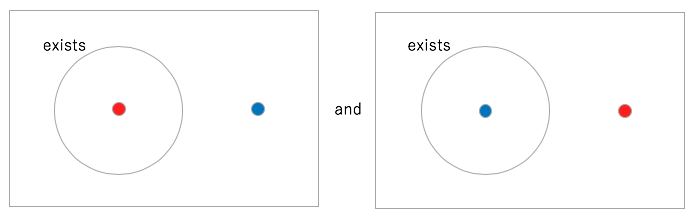
\includegraphics[clip,width=10cm]{./T1.png}
                        \caption{$T_1$ space}
                    \end{center}
                \end{figure}
            
            \item $T_2$ : Hausdorff space $(X,\ \mathfrak{O})$ \\
                $$\forall x,\ y \in X,\ \exists V_x \in V(x),\ \exists V_y \in V(y) \ s.t. \ V_x \cap V_y \neq \phi $$
                \begin{figure}[H]
                    \begin{center}
                        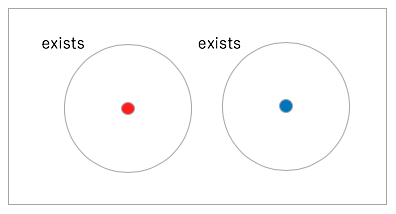
\includegraphics[clip,width=6cm]{./T2.png}
                        \caption{$T_2$ space}
                    \end{center}
                \end{figure}
            
            \item $T_{2 \frac{1}{2}}$ : Urysohn space $(X,\ \mathfrak{O})$ \\
                $$\forall x,\ y \in X,\ \exists V_x \in V^*(x),\ \exists V_y \in V^*(y) \ s.t. \ V_x \cap V_y \neq \phi$$
                $$V^*(x) : \text{closed neighborhood of } x,\ V^*(y) : \text{closed neighborhood of } y$$
                \begin{figure}[H]
                    \begin{center}
                        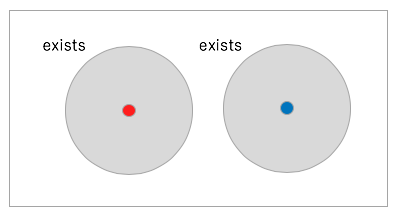
\includegraphics[clip,width=6cm]{./T2_2.png}
                        \caption{$T_{2 \frac{1}{2}}$ space}
                    \end{center}
                \end{figure}
            
            \item completely $T_{2}$ : Completely Hausdorff space $(X,\ \mathfrak{O})$ \\
                $$\forall x,\ y \in X,\ \exists f : X \mapsto [0,\ 1],\ s.t. \ f(x) = 0,\ f(y) = 1,\ f \text{ is continuous function.}$$
            
            \item $T_{3}$ : Regular Hausdorff space $(X,\ \mathfrak{O})$ \\
                Regular Hausdorff space is a topological space that is both regular and a Hausdorff space. \\
                Regular space : $$\forall F \text{ (closed set) },\ \forall x \notin F ,\ \exists O_1,\ O_2 \ s.t. \ x \in O_1,\ F \subset O_2,\ O_1 \cap O_2 = \phi $$
                \begin{figure}[H]
                    \begin{center}
                        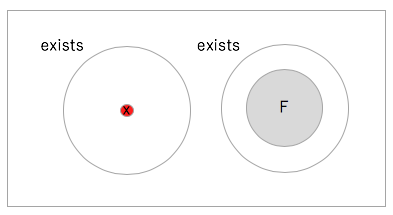
\includegraphics[clip,width=6cm]{./T3.png}
                        \caption{Regular space}
                    \end{center}
                \end{figure}

            \item $T_{3 \frac{1}{2}}$ : Tychonoff space (completely regular Hausdorff space) $(X,\ \mathfrak{O})$ \\
                Regular Hausdorff space is a topological space that is both conmpletely regular and a Hausdorff space. \\
                Completely regular space : $\forall A \subseteq X,\ A \text{ is closed set},\ \forall x \in X \backslash A,$\\
                $$ \exists f : X \mapsto \mathbb{R} \ s.t. \ f(x) = 1,\ f(a) = 0 (\forall a \in A),\ f \text{ is continuous function.}$$
            
            \item $T_{4}$ : Normal Hausdorff space $(X,\ \mathfrak{O})$ \\
                Normal Hausdorff space is a topological space that is both normal and a Hausdorff space. \\
                Normal space : $$\forall E,\ F \text{ :closed set},\ \exists O_1,\ O_2 \ s.t. \ E \subset O_1,\ F \subset O_2,\ O_1 \cap O_2 = \phi$$
                \begin{figure}[H]
                    \begin{center}
                        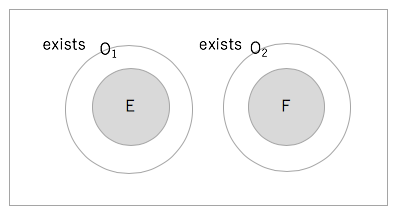
\includegraphics[clip,width=6cm]{./T4.png}
                        \caption{Normal space}
                    \end{center}
                \end{figure}
            \item $T_5$ : Completely Normal Hausdorff space $(X,\ \mathfrak{O})$ \\
                Completely Normal Hausdorff space is a topological space that is both completely normal and Hausdorff space. \\
                Completely Normal space : $$\forall A \subset X,\ ( A,\ \mathfrak{O}_{A}) \text{ is normal space.} $$
            
            %\item $T_6$ : Perfectly normal Hausdorff $(X,\ \mathfrak{O})$ \\
            %Perfectly normal Hausdorff space is a topological space that is both Perfectly normal and Hausdorff space. \\
            %Perfectly normal space : $$ $$

        \end{enumerate}

        
    

    \item[\bf{Definition:}] Metrizable space (距離化可能空間) \\
        A topological space $(X,\ \mathfrak{O})$ is said to be metrizable if there is a metric:
        $$ d: X \times X \mapsto [0,\ \infty) $$
        such that the topology induced by $d$ is $\mathfrak{O}$.

    \item[\bf{Theorem:}] Urysohn's metrization theorem (距離化可能定理) \\
        $$ \text{Hausdorff second-countable regular space is metrizable.} $$
        
    

\end{description}
\end{document}